\chapterimage{chapter_head_1.pdf} 
\chapter{Sistema de memoria gráfica de la NDS}

Este capítulo trata sobre la realización de videojuegos con gráficos en la consola NDS. Este documento se ha redactado usando como principal fuente los capítulos 7, 8 y 9 del libro: Francisco Moya Fernández y María José Santofimia Romero. \textit{Laboratorio de Estructura de Computadores empleando videoconsolas Nintendo DS}. UCLM, ISBN: 978-84-9981-039-4.

% -----------------------------------------------------
% -----------------------------------------------------
% -----------------------------------------------------
% -----------------------------------------------------
\section{Introducción}
El hardware de vídeo de la Nintendo DS se compone de dos núcleos gráficos 2D, uno principal o \textit{main} y otro secundario o \textit{sub}, diferenciados únicamente en que el motor principal puede renderizar tanto la memoria de vídeo virtual sin utilizar el motor 2D, como mapas de bits de 256 colores, así como utilizar el motor 3D para el renderizado de alguno de sus fondos. 

El concepto de fondo es básico para comprender cómo funcionan los modos de vídeo de la Nintendo DS y se puede entender como un concepto equivalente al de capa o layer utilizado por algunas aplicaciones de diseño gráfico para facilitar la composición de una imagen a partir de la superposición del contenido de las capas. Los núcleos gráficos de la Nintendo DS disponen de cuatro fondos, etiquetados como \textit{BG0}, \textit{BG1}, \textit{BG2} y \textit{BG3}, cuya configuración dependerá del tipo de gráfico a representar.

Un modo gráfico básicamente agrupa un conjunto de configuraciones para cada uno de los fondos. La Figura \ref{fig_c5_modulos} resume los modos disponibles para el núcleo principal y el secundario. Los seis primeros modos, \textit{Mode 0} a \textit{Mode 5}, son comunes para los dos núcleos. Además, el núcleo principal cuenta con el \textit{Mode }6 y con el modo \textit{frame buffer}.

\begin{figure}[t]
	\centering
	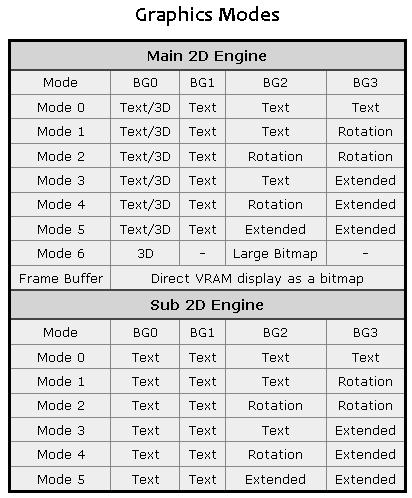
\includegraphics[height=9cm]{Figuras/C5/c5_modos-graficos.png}
	\caption{Modulos gráficos}
	\label{fig_c5_modulos}
\end{figure}

Existen tres tipos diferentes de configuraciones para los fondos 2D, que son \textit{Text}, \textit{Rotation} y \textit{Extended Rotation} y el modo \textit{framebuffer} que pinta la imagen directamente sin utilizar fondos. A los modos \textit{Text} también se les llama modos teselados, y a los modos \textit{Rotation} también se les conoce como modos \textit{Rotoscale}.

Las imágenes que se desean mostrar en la pantalla deben ser traducidas a contenido binario, que se guardará junto con el programa y que debe ser copiado en un \textit{banco de memoria VRAM (Video RAM)} que es donde está mapeada la pantalla. Mapear la pantalla a un banco de memoria significa que a la pantalla se le asigna ese banco de memoria, de forma que lo que se haya escrito en ese banco de memoria será lo que se vea en la pantalla. 

La Nintendo DS tiene 9 bancos de memoria de vídeo, que se pueden usar con diferentes propósitos. Cada de uno de estos bancos de memoria está etiquetado desde \textit{VRAM\_A} hasta \textit{VRAM\_I}. La Tabla \ref{tab_c5_vram} muestra cada uno de los bancos de memoria VRAM con su tamaño y su dirección de memoria. La cantidad total de memoria de vídeo es de 656KB. 

\begin{table}[t]
\centering
\caption{Tamaño y dirección de memoria de cada banco de memoria.}
\begin{tabular}{|l |c | c|}
\hline
Banco & Tamaño &  Dirección memoria  \\
\hline
\hline
VRAM\_A & 128KB & 0x6800000 \\
\hline
VRAM\_B & 128KB  &	0x6820000 \\
\hline
VRAM\_C & 128KB  &	0x6840000 \\
\hline
VRAM\_D	& 128KB  &	0x6860000 \\
\hline
VRAM\_E	& 64KB  &	0x6880000\\
\hline
VRAM\_F	& 16KB  &	0x6890000 \\
\hline
VRAM\_G	& 16KB  &	0x6894000\\
\hline
VRAM\_H	& 32KB & 	0x6898000 \\
\hline
VRAM\_I	& 16KB  &	0x68a0000\\
\hline
\end{tabular}
\label{tab_c5_vram}
\end{table}

La Figura \ref{fig_c5_vram} muestra los bancos de memoria que se pueden usar en cada motor gráfico y para que fin. Por ejemplo, el banco \textit{VRAM C} se puede usar tanto por el motor \textit{main} como por el \textit{sub}. Sin embargo, el banco \textit{VRAM A} solo puede ser usado por el motor \textit{main}.

\begin{figure}[t]
	\centering
	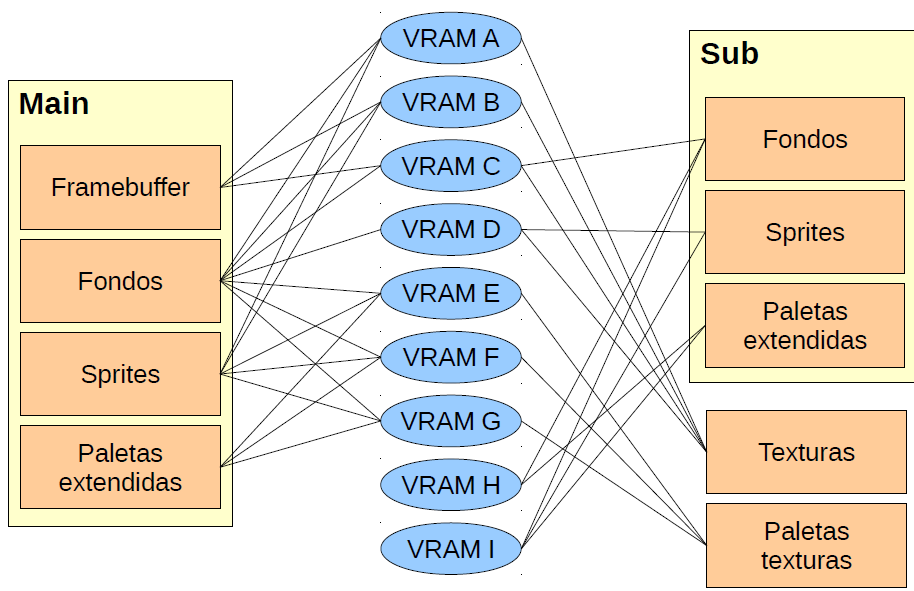
\includegraphics[height=9cm]{Figuras/C5/c5_vram.png}
	\caption{Bancos de memoria y que motores, y para que fin, los pueden usar.}
	\label{fig_c5_vram}
\end{figure}
% -------------------------------------------------------------
% -------------------------------------------------------------
\section{El registro \textit{REG\_POWERCNT}} 
El registro \textit{REG\_POWERCNT} es el encargado del encendido de todo el hardware gráfico. La Figura \ref{c5_bits_reg_powercnt} muestra el significado de algunos de sus bits. El contenido de este registro permite activar ambas pantallas y los dos motores gráficos: el principal (\textit{main}) y el secundario (\textit{sub}) para trabajar en 2D. Además, el bit 15  permite intercambiar ambas pantallas y asignar el motor principal a la pantalla superior (top) en vez de a la inferior que es la que tiene por defecto.

\begin{figure}[h]
\centering
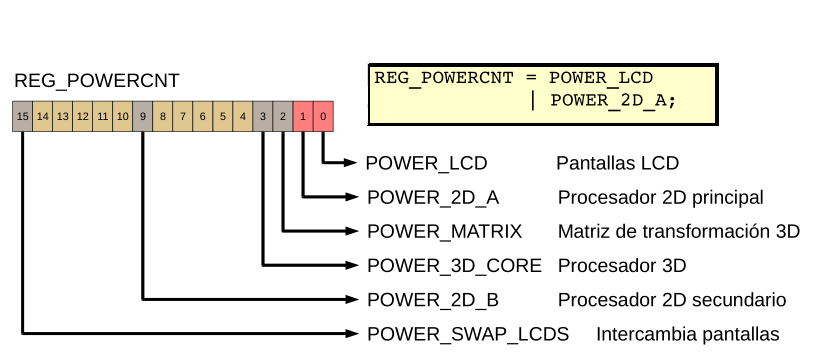
\includegraphics[height=6cm]{Figuras/C5/c5_reg_powercnt.png}
\caption{Significado de los bits del registro \textit{REG\_POWERCNT}}
\label{c5_bits_reg_powercnt}
\end{figure}

Por ejemplo, para activar ambas pantallas y únicamente el motor principal se puede usar la instrucción:
\begin{verbatim}
REG_POWERCNT = POWER_LCD | POWER_2D_A;
\end{verbatim}

Para activar ambas pantallas y ambos motores se puede usar la instrucción:
\begin{verbatim}
REG_POWERCNT = POWER_LCD | POWER_2D_A | POWER_2D_B;
\end{verbatim}

Se puede encontrar más información en la web: \url{http://libnds.devkitpro.org/system_8h.html}. 



% -------------------------------------------------------------
% -------------------------------------------------------------
\section{El registro \textit{REG\_DISPCNT}} 
El registro \textit{REG\_DISPCNT} es el que se encarga de controlar los modos y fondos activos. La Figura \ref{fig_c5_reg_dispcnt3} muestra el significado de algunos de sus bits. Cabe destacar la finalidad de los siguientes bits:

\begin{itemize}
	\item Bits 0-2: especifican el modo gráfico. Del 0 al 6 en binario con tres bits.
	\item Bits 8-12: especifican el fondo.
	\item Bits 17-19: especifican la configuración del modo gráfico \textit{framebuffer}.
\end{itemize}

\begin{figure}[t]
\centering
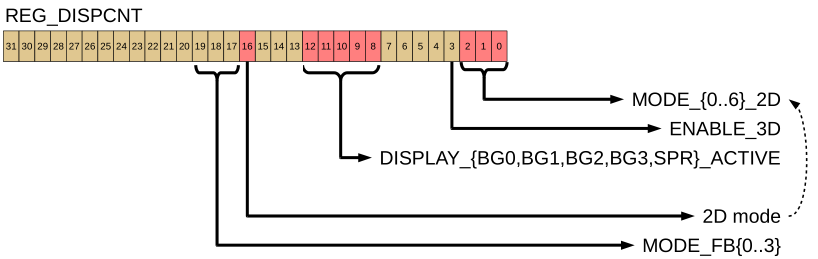
\includegraphics[height=4cm]{Figuras/C5/c5_reg_dispcnt3.png}
\caption{Significado de los bits del registro \textit{REG\_DISPCNT}}
\label{fig_c5_reg_dispcnt3}
\end{figure}

Por ejemplo, para indicar que se activa el \textit{Modo 0} con el fondo \textit{BG0} en el motor \textit{main}, se debe usar la siguiente instrucción:

\begin{verbatim}
REG_DISPCNT = MODE_0_2D | DISPLAY_BG0_ACTIVE;
\end{verbatim}

Para el motor secundario se usará la siguiente instrucción:

\begin{verbatim}
REG_DISPCNT_SUB = MODE_0_2D | DISPLAY_BG0_ACTIVE;
\end{verbatim}

Esta operación también se puede llevar a cabo, en el motor \textit{main}, mediante la instrucción:
\begin{verbatim}
videoSetMode(MODE_0_2D);
\end{verbatim}

Para el motor \textit{sub}, habrá que usar la instrucción:
\begin{verbatim}
videoSetModeSub(MODE_0_2D);
\end{verbatim}

Se puede encontrar más información en la web: \url{http://libnds.devkitpro.org/video_8h.html}. 


% -------------------------------------------------------------
% -------------------------------------------------------------
\section{Los registros \textit{VRAM\_?\_CR}} 
Cada \textit{banco VRAM} tiene un registro \textit{VRAM\_?\_CR} (donde ? puede tomar los valores de A a I) para activarlo y seleccionar su función. La Figura \ref{fig_c5_reg_vram1} muestra el significado de cada uno de sus bits. Cabe destacar que los bits etiquetados con \textit{Modo} y \textit{Desplazamiento} son los que permiten seleccionar la función del fondo configurado en el registro \textit{REG\_DISPCNT}. Por su parte el \textit{bit 7} es el que permite activar el correspondiente \textit{banco VRAM}.

\begin{figure}[t]
\centering
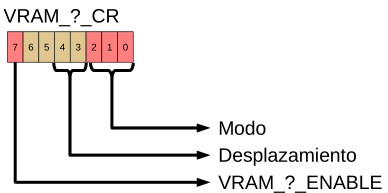
\includegraphics[height=4cm]{Figuras/C5/c5_reg_vram1.png}
\caption{Significado de los bits del registro \textit{VRAM\_?\_CR}}
\label{fig_c5_reg_vram1}
\end{figure}

Como ejemplo, para indicar que se activa \textit{VRAM\_A} y que se asigna a fondos del motor principal (\textit{main}) se debe usar la instrucción:

\begin{verbatim}
VRAM_A_CR = VRAM_ENABLE | VRAM_A_MAIN_BG;
\end{verbatim}

Para el motor secundario se usará la siguiente instrucción:

\begin{verbatim}
VRAM_C_CR = VRAM_ENABLE | VRAM_C_SUB_BG;
\end{verbatim}

En este caso se activa la \textit{VRAM C}, puesto que el motor secundario no puede usar la \textit{VRAM A} (ver figura \ref{fig_c5_vram}).
